\documentclass[10pt, a4paper,spanish]{article}

\usepackage[utf8]{inputenc}
\usepackage[spanish]{babel}

\usepackage[T1]{fontenc}

\usepackage[hmarginratio=1:1,top=32mm,columnsep=20pt]{geometry}
\usepackage[hang, small,labelfont=bf,up,textfont=it,up]{caption}

\usepackage{float}

\usepackage{amsmath}

\usepackage{enumitem}

\usepackage{graphicx}
\graphicspath{ {images/} }


\usepackage{titlesec}
\renewcommand\thesection{\Roman{section}}
\renewcommand\thesubsection{\Roman{subsection}}
\titleformat{\section}[block]{\large\scshape\centering}{\thesection.}{1em}{}
\titleformat{\subsection}[block]{\large}{\thesubsection.}{1em}{}

\usepackage{fancyhdr}
\pagestyle{fancy}
\fancyhead{}
\fancyfoot{}
\fancyhead[C]{ \today \ $\bullet$ Ingeniería del Conocimiento $\bullet$ Clips 1}
\fancyfoot[RO]{\thepage}

%-------------------------------------------------------------------------------
%	TITLE SECTION
%-------------------------------------------------------------------------------

\title{\vspace{-15mm}\fontsize{24pt}{10pt}\selectfont\textbf{Clips 1}} % Article title

\author{
	Fernández Angulo, Óscar \\
	\and
	García Prado, Sergio
}

\date{\today}

\setcounter{section}{2} % Sections will start at 3

%-------------------------------------------------------------------------------
\begin{document}

	\maketitle % Insert title

	\thispagestyle{fancy} % All pages have headers and footers


%-------------------------------------------------------------------------------
%	TEXT
%-------------------------------------------------------------------------------



    \section{La figura muestra un fragmento de una red causal que modela conocimiento del dominio para la tarea de diagnosis en el dominio de los automóviles. La red asocia posibles causas de fallo (fusible fundido, batería baja o depósito de combustible vacío) con estados intermedios (potencia, combustible en motor y síntomas comportamiento motor, inspección fusible, indicador batería...).}

		\begin{figure}[H]
			\begin{center}
				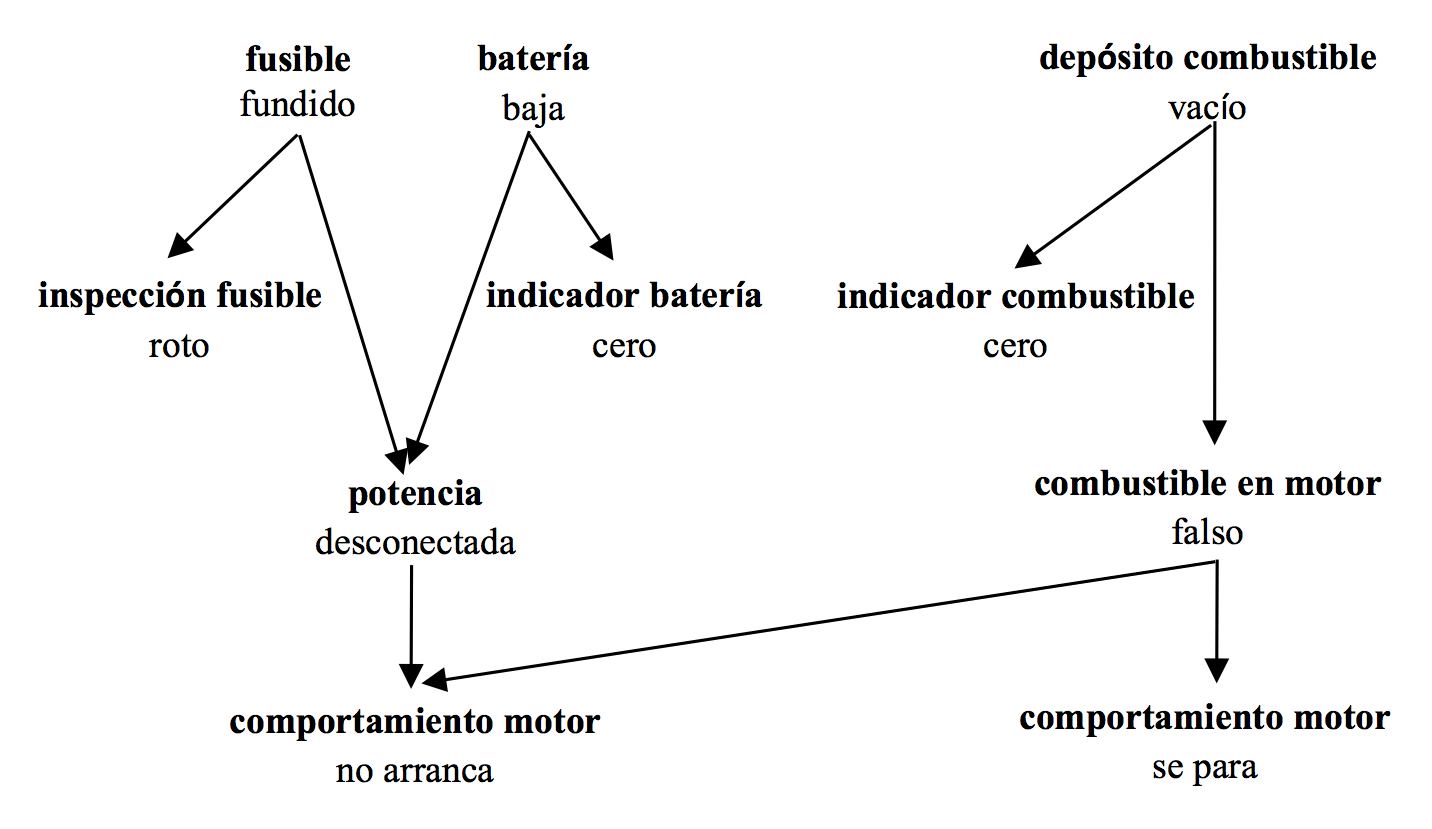
\includegraphics[width=0.75\textwidth]{exercise-3-network}
			\end{center}
		\end{figure}

		\paragraph{}
		La base de conocimiento necesaria para representar el problema requiere de un conjunto tanto de objetos como de atributos de los mismos. Esto se describe a continuación a partir de la Definición del Dominio (DD), el cual se compone del conjunto de Objetos (O) y la Definición de Atributos (DA):

		\begin{equation*}
			O = \{coche, motor, potencia, bateria, fusible, combustible, deposito \}
		\end{equation*}

		\begin{multline*}
			DA = \{ \\
				coche.sePara^s:boolean \\
				motor.arranca^s:boolean, motor.combustible^s:boolean, \\
				potencia.conectada^s:boolean \\
				bateria.indicador^s:number, bateria.estado^s,\\
				fusible.inspeccion^s, fusible.estado^s, \\
				combustible.indicador^s:number, \\
				deposito.estado^s \\
			\}
		\end{multline*}

		\paragraph{}
		A continuación se describe el conjunto de reglas de la base de conocimiento:

		\begin{enumerate}[label={\textbf{R\theenumi:}}]

			\item
				\textbf{if} $equals(motor, arranca, false)$ \\
				\textbf{then} $add(potencia, conectada, false)$ \textbf{fi}
				\\ \\
				En el caso de que el motor no arranque, significa que no está conectada la potencia.

			\item
				\textbf{if} $equals(motor, arranca, false)$ \\
				\textbf{then} $add(motor, combustible, false)$ \textbf{fi}
				\\ \\
				Si el motor no arranca otra de las posibles causas es que no tenga combustible.

			\item
				\textbf{if} $equals(coche, sePara, true)$ \\
				\textbf{then} $add(motor, combustible, false)$ \textbf{fi}
				\\ \\
				La causa de que el coche se haya parado viene dada por la falta de combustible en el motor.

			\item
				\textbf{if} $equals(potencia, conectada, false)$ \textbf{and} $equals(fusible, inspeccion, roto)$ \\
				\textbf{then} $add(fusible, estado, fundido)$ \textbf{fi}
				\\ \\
				Si la potencia no está conecta y la inspección del fusible determina que este está roto entonces se puede determinar que el estado del fusible es fundido.

			\item
				\textbf{if} $equals(potencia, conectada, false)$ \textbf{and} $equals(bateria, indicador, 0)$ \\
				\textbf{then} $add(bateria, estado, baja)$ \textbf{fi}
				\\ \\
				Si la potencia no está conectada y la batería indica el valor cero entonces el estado de la batería es baja.

			\item
				\textbf{if} $equals(motor, combustible, false)$ \textbf{and} $equals(combustible, indicador, 0)$ \\
				\textbf{then} $add(deposito, estado, vacio)$ \textbf{fi}
				\\ \\
				Si no llega combustible al motor y además el indicador de compustible indica el valor cero entronces el resultado es que el depósito está vacío.


		\end{enumerate}



	\clearpage
	\section{Considerar el asistente al diagnostico propuesto por Pool y Mackworth}

		\begin{figure}[H]
			\begin{center}
				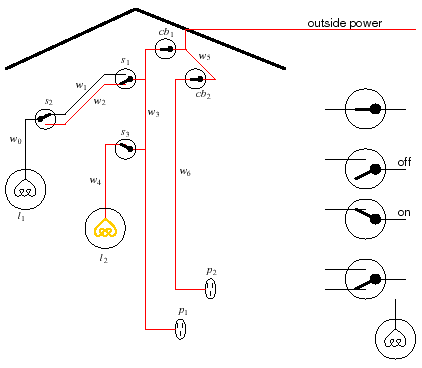
\includegraphics[width=0.6\textwidth]{diagnostic-assistant}
			\end{center}
		\end{figure}

		\subsection{Ontología General}

			\paragraph{}
			La base de conocimiento necesaria para representar el problema requiere de un conjunto tanto de objetos como de atributos de los mismos. Mientras que el conjunto de objetos se ha referenciado de forma particular, la declaración de atributos (DA) se ha dejado especificada de manera general para poder ser aprovechada para su reutilziación en otros problemas utilizando subíndices:

			\begin{equation*}
				O = \{l_1, l_2, p_1, p_2, s_1, s_2, s_3, cb_1 cb_2, w_1, w_2, w_3, w_4, w_5, w_6, outside\}
			\end{equation*}

			\begin{multline*}
				DA = \{ \\
					l_i.live^s:boolean, l_i.type^s, l_i.lit^s:boolean, l_i.ok^s:boolean, \\
					p_i.live^s:boolean, p_i.type^s, p_i.electrize^s:boolean, p_i.ok^s:boolean, \\
					s_j.live^s:boolean, s_j.type^s, s_j.state^s:{up, down}, s_j.up^s, s_j.down^s, s_j.ok^s:boolean, \\
					cb_k.live^s:boolean, cb_k.type^s, cb_k.ok^s:boolean, cb_k.connected^s, \\
					w_l.live^s:boolean, w_l.type^s, w_l.ok^s:boolean, w_l.connected^m, \\
					outside.live^s:boolean, outside.ok^s:boolean, outside.connected^s \\
				\}
			\end{multline*}

			\begin{equation*}
				DD = O \cup DA
			\end{equation*}

			\paragraph{}
			A continuación se muestran el conjunto de reglas necesarias para llevar a cabo la produción de conocimiento y por lo tanto, la modificación de la memoria de trabajo (MT), que en un estado inicial será inicializada a partir del conjunto de hechos indicados en la Ontología Especifica, tal y como se describirá próximamente.

			\begin{enumerate}[label={\textbf{R\theenumi:}}]
				\item
					\textbf{if} $equals(?x, connected, ?y)$ \textbf{and} $equals(?x, live, t)$ \textbf{and} $equals(?x, ok, t)$ \\
					\textbf{then} $add(?y, live, t)$ \textbf{fi}

				\item
					\textbf{if} $equals(?x, type, ligth)$ \textbf{and} $equals(?x, live, t)$ \textbf{and} $equals(?x, ok, t)$ \\
					\textbf{then} $add(?x, lit, t)$ \textbf{fi}

				\item
					\textbf{if} $equals(?x, type, power\_outlet)$ \textbf{and} $equals(?x, live, t)$ \textbf{and} $equals(?x, ok, t)$ \\
					\textbf{then} $add(?x, electrize, t)$ \textbf{fi}

				\item
					\textbf{if} $equals(?x, type, switch)$ \textbf{and} $equals(?x, live, t)$ \textbf{and} $equals(?x, state, up)$ \\
					\hspace*{0.5cm} \textbf{and} $equals(?x, up, ?y)$ \\
					\textbf{then} $add(?y, live, t)$ \textbf{fi}

				\item
					\textbf{if} $equals(?x, type, switch)$ \textbf{and} $equals(?x, live, t)$ \textbf{and} $equals(?x, state, down)$ \\
					\hspace*{0.5cm} \textbf{and} $equals(?x, down, ?y)$ \\
					\textbf{then} $add(?y, live, t)$ \textbf{fi}
			\end{enumerate}


		\subsection{Ontología Específica}

			\begin{equation*}
				\begin{split}
					l_1.type=ligth, l_1.ok=true, \\
					l_2.type=ligth, l_2.ok=true, \\
					p_1.type=power\_outlet, p_1.ok=true, \\
					p_2.type=power\_outlet, p_2.ok=true, \\
					s_1.type=switch, s_1.state=down, s_1.up=w_1, s_1.down=w_2, s_1.ok=true, \\
					s_2.type=switch, s_2.state=up, s_2.up=w_1, s_2.down=w_2, s_2.ok=true, \\
					s_3.type=switch, s_3.state=up, s_3.up=w_4, s_3.ok=true, \\
					cb_1.type=circuit_breaker, cb_1.connected=w_3, cb_1.ok=true,\\
					cb_2.type=circuit_breaker, cb_2.connected=w_6, cb_2.ok=true,\\
					w_0.type=wire, w_1.ok=true, w_0.connected=l_1,\\
					w_1.type=wire, w_1.ok=true, \\
					w_2.type=wire, w_2.ok=true, \\
					w_3.type=wire, w_3.ok=true, w_3.connected=\{s_1, s_3, p1\}, \\
					w_4.type=wire, w_4.ok=true, w_4.connected=l_2, \\
					w_5.type=wire, w_5.ok=true, w_5.connected=\{cb_1, cb_2\}, \\
					w_6.type=wire, w_6.ok=true, w_6.connected=p2, \\
					outside.live=true, outside.ok=true, outside.connected=w_5
				\end{split}
			\end{equation*}


\end{document}
